\documentclass[12pt]{article}
\special{papersize=3in,5in}
\usepackage[T1]{fontenc}
\usepackage[utf8x]{inputenc}
\usepackage[type1]{libertineRoman}
\usepackage[type1]{biolinum}
\usepackage[type1]{libertineMono}
\usepackage[libertine]{newtxmath}
\renewcommand{\familydefault}{\sfdefault}
\usepackage{graphicx}
\usepackage{amssymb,amsmath, amsfonts}
\usepackage{booktabs}
\usepackage{color}
\usepackage[dvipsnames]{xcolor}
\usepackage{multirow}
\usepackage{rotating}
\usepackage{graphicx}
\usepackage{wasysym}
\usepackage{hyperref}
\hypersetup{
    colorlinks=true, % make the links colored
    linkcolor=NavyBlue, % color TOC links in blue
    urlcolor=red, % color URLs in red
    linktoc=all % 'all' will create links for everything in the TOC
}
\usepackage{mathrsfs} % https://www.ctan.org/pkg/mathrsfs%
\graphicspath{ {./images/} }

\title{
Teoria Analisi\\
parte 2\\}
\author{}
\date{2019-2020}
\renewcommand*\contentsname{Indice}
\begin{document}

\maketitle

\tableofcontents

\newpage

\section{Continuità}

\subsection{Continuità in un punto, in un insieme}

Sia \(f: I \rightarrow \mathbb{R}\), \(I\) intervallo, e
\(x_0 \in I\) un punto di accumulazione per I
si dice che $f$ è continua in $c$ se esiste
\[  \lim_{x \to x_0} f(x) = f(x_0)\]
Si dice che $f$ è continua in $I$ se è continua in ciascun punto di $I$.

\subsection{Punti di discontinuità}

\subsubsection{I specie (o di salto)}
Sia $x_0 \in I$ un punto di accumulazione per $I$
e supponiamo che $f$ sia definita in un intorno
circolare di $x_0$. Diciamo che la funzione $f$ ha
in $x_0$ un punto di discontinuità di prima specie
(o di salto) se esistono finiti:
\[ \lim_{x \to x_{0}^{+}} f(x) \neq \displaystyle \lim_{x \to x_{0}^{-}} f(x) \]

\subsubsection{II specie}
Sia $x_0 \in I$ un punto di accumulazione per $I$
e supponiamo che $f$ sia definita in un intorno
circolare di $x_0$. Diciamo che la funzione $f$ ha
in $x_0$ un punto di discontinuità di seconda specie se:
\[ \lim_{x \to x_{0}^-} \begin{cases} \nexists \\
= \infty \end{cases} \hspace{0.5cm} \vee \hspace{0.5cm} \lim_{x \to x_{0}^+} \begin{cases} \nexists \\
= \infty \end{cases} \]

\subsubsection{III specie (o eliminabile)}
Sia $x_0 \in I$ un punto di accumulazione per $I$
e supponiamo che $f$ sia definita in un intorno
circolare di $x_0$. Diciamo che la funzione $f$ ha
in $x_0$ un punto di discontinuità di terza specie
(o eliminabile) se esiste finito:
\[  \lim_{x \to x_0} f(x) = l \neq f(x_0) \]
Si ottiene una funzione $\tilde{f}$ continua in $x_0$
estendendo o modificando $f$:
\[ \tilde{f}(x) := \begin{cases} \begin{aligned}
f(x)\quad \text{se} \; x\ \neq x_0 \\
l\quad \text{se} \; x\ = x_0
\end{aligned}  \end{cases} \]


\subsection{Discontinuità delle funzioni monotone}
Sia $f: (a, b) \to \mathbb{R}$ monotona. Allora,
per il teorema di monotonia,
i limiti destro e sinistro di $f$
esistono finiti per ogni $x \in (a,b)$.
Per cui una funzione monotona
può solo avere discontinuità
di prima specie (o di salto).

\subsection{Teorema di Weierstrass}
Sia $f$ una funzione continua su un intervallo
chiuso e limitato $[a,b]$. Allora $f$ è limitata
su $[a,b]$ e ivi assume valori minimo e massimo.
Cioè esistono $x_m$,$x_M \in [a,b]$ tali che
\[ f(x_m) \leq f(x) \leq f(x_M) \hspace{0.3cm} \forall x \in [a,b]\]
Si dice che $x_m$ è punto di minimo per $f$,
ed $m = f(x_m)$ è il minimo di $f$;
analogamente, $x_M$ è punto di massimo per $f$,
ed $M = f(x_M)$ è il massimo di $f$.

\subsection{Teorema degli zeri (*)}

Sia $f \in \mathscr{C}([a,b])$ tale che $f(a)\cdot f(b)<0$. Allora $\exists c \in (a,b)$ tale che $f(c) = 0$ \newline
\textbf{Dimostrazione} \newline
Supponiamo che $f(a) > 0$. Prendiamo $c_1 = \frac{a+b}{2}$, punto medio di $[a,b]$. Se $f(c_1)=0$, il teorema è dimostrato. Se $f(c_1) \neq 0$, consideriamo l'intervallo $[a_1, b_1]$ e procediamo nel modo seguente:
\begin{itemize}
  \item se $f(c_1) < 0$, allora $a_1 = a, b_1 = c_1$
  \item se $(c_1) > 0$, allora $a_1 = c_1, b_1 = b$
\end{itemize}
E avremo che 
\[ f \in \mathscr{C}([a_1,b_1]) \]
\[b_1 - a_1 = \frac{b-a}{2}\]
\[a<a_1\] 
\[b>b_1\]
Analogamente, poniamo $c_2 = \frac{b_1 + a_1}{2}$, punto medio di $[a_1,b_1]$. Se $f(c_2)=0$, il teorema è dimostrato. Se $f(c_2) \neq 0$, consideriamo l'intervallo $[a_2, b_2]$ e procediamo nel modo seguente:
\begin{itemize}
  \item se $f(c_2) < 0$, allora $a_2 = a_1, b_2 = c_2$
  \item se $(c_2) > 0$, allora $a_2 = c_2, b_2 = b_1$
\end{itemize}
E avremo che
\[ f \in \mathscr{C}([a_2,b_2]) \]
\[b_2 - a_2 = \frac{b-a}{2^2}\]
\[a_1<a_2\] 
\[b_1>b_2\]
Continuando in questo modo troviamo infiniti intervalli $[a_n, b_n]$
con le seguenti proprietà
\[
a_n \leq a_{n+1} \quad \text{e} \quad b_n \geq b_{n+1}
\]
\[ f \in C([a_n,b_n]) \]
\[ b_n - a_n = \frac{b-a}{2^n} \] 
\[ f(a_n)>0 \quad \text{e} \quad f(b_n) < 0 \]
\newpage
Essendo ${a_n}\uparrow$ e ${b_n}\downarrow$, esistono finiti i limiti:
\[ \lim_{n \to +\infty} a_n = c \in [a,b] \]
\[ \lim_{n \to +\infty} b_n = \lim_{n \to +\infty} a_n + \frac{b-a}{2^n} = c \]
Inoltre, poiché $f \in C([a,b])$
\[ \lim_{n \to +\infty} f(a_n) = f(c)\quad \text{quindi} f(a_n) >0 \Rightarrow f(c) \geq 0 \]
\[ \lim_{n \to +\infty} f(b_n) = f(c) \quad \text{quindi} f(b_n) <0 \Rightarrow f(c) \geq 0 \]
quindi $f(c) = 0$

\subsection{Teorema dei valori intermedi (*)}
Sia $f \in \mathscr{C}(I)$, $I$ intervallo, e sia $\lambda \in (Inf f, Sup f)$.
Allora $\exists x \in I\ |\ f(x) = \lambda$.\newline
\textbf{Dimostrazione} \newline
Siano $x_1 < x_2$,\ $\lambda \in (Inf f, Sup f)$
\[ \lambda > Inf f \Rightarrow \exists x_1 \in I\ f(x_1) < \lambda \]
\[ \lambda < Sup f \Rightarrow \exists x_2 \in I\ f(x_2) > \lambda \]
Considero $[x_1,x_2]$ e una funzione $g \in C([x_1,x_2]), g(x) = f(x) - \lambda$\\
Allora 
\[g(x_1) = f(x_1) - \lambda < 0\] 
\[g(x_2) = f(x_2) - \lambda > 0\]
Per il teorema degli zeri,
\[\exists c: \hspace*{0.1cm} g(c) = f(c) - \lambda = 0 \]
\[\quad f(c) = \lambda \]

\subsection{Asintoti}
\subsubsection{Asintoto verticale}
Sia $f: Dom(f) \subseteq \mathbb{R} \to \mathbb{R}$ e sia
$x_0$ un punto di accumulazione per $Dom(f)$.
Si dice che $f$ ha un asintoto verticale
per $x \to x_0$ di equazione $x = x_0$
se esiste \[ \lim_{x \to x_0} f(x) = \infty\]

\subsubsection{Asintoto orizzontale}
Sia $f: Dom(f) \subseteq \mathbb{R} \to \mathbb{R}$ e
supponiamo che il suo dominio sia illimitato.
Si dice che $f$ ha un asintoto orizzontale
di equazione $y = l\ (l \in \mathbb{R})$
se esiste \[ \lim_{x \to \infty} f(x) = l\]
\subsubsection{Asintoto obliquo}
Sia $f: Dom(f) \subseteq \mathbb{R} \to \mathbb{R}$ e\\
supponiamo che il suo dominio sia illimitato.
Si dice che $f$ ha un asintoto obliquo
di equazione
\[ y = mx+q \quad (m, q \in \mathbb{R}, \quad m \neq 0)\quad \text{per} \quad  x \to \pm \infty \]
se esistono
\[ \lim_{x \to \infty} \frac{f(x)}{x} = m \neq 0 \]
\[ \lim_{x \to \infty} [f(x) - mx] = q \]

\subsection{Continuità di funzione inversa}
Sia $f: I \to \mathbb{R}$, con $I$ intervallo,
una funzione continua in $I$. Allora $f$ è invertibile
in $I$ se e solo se è strettamente monotona.
In tal caso, la sua inversa è ancora strettamente
monotona e continua.

\section{Calcolo differenziale}

\subsection{Definizione di derivata}
Sia $f: (a,b) \to \mathbb{R}$; $f$ si dice
derivabile in $x_0 \in (a,b)$ se esiste finito
\[ \lim_{h \to 0} \frac{f(x_0 +h) - f(x_0)}{h}=k\]
Il limite $l$ prende il nome di "derivata di $f$ in $x_0$"\\
e si indica con:
\[ f'(x_0) \quad \left. \frac{df}{dx} \right |_{x = x_0} \quad  Df(x_0) \quad \dot{f}(x_0) \]
\\
OSS:
\[ \lim_{h \to 0} \frac{f(x_0 +h) - f(x_0)}{h} = \lim_{x \to x_0} \frac{f(x) - f(x_0)}{x - x_0} = f'(x_0)\]

\subsubsection{Significato geometrico della derivata}
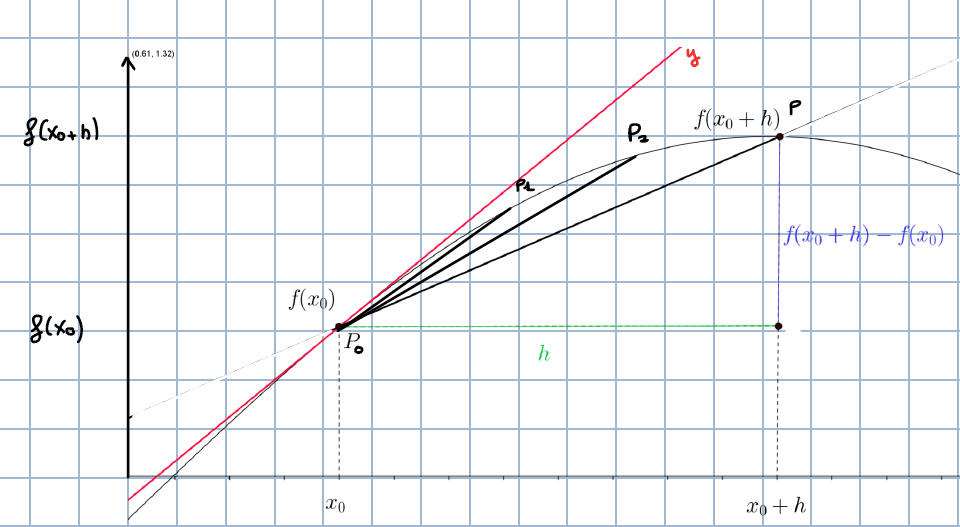
\includegraphics[width=\textwidth]{images/deriv.png}
La retta $y=f(x_0) + f'(x_0)(x-x_0)$ è la retta
tangente al grafico di f nel punto $P_0 = (x_0, f(x_0))$
\[  \lim_{h \to 0} \frac{f(x_0 + h) - f(x_0)}{h} = f'(x_0)
\Leftrightarrow
f(x_0 + h) - f(x_0) = f'(x_0)h + \sigma(h) \quad h \to 0\]
ossia, scrivendo $h$ come $h = x - x_0$
\[ f(x) - f(x_0) = f'(x_0)(x-x_0) + \sigma(x-x_0) \quad  \ x \to x_0\]

\subsection{Derivabilità e continuità}
Se $f$ è derivabile in un punto $x_0$
allora $f$ è continua in $x_0$. Non è vero il contrario,
ossia che se $f$ è continua in $x_0$ allora è
derivabile in $x_0$ (esempio: $f(x) = |x|$, $x_0 = 0$)

\subsection{Derivata di funzione composta}
Sia $g \circ f$ la composta di due funzioni $f$ e $g$. Se $f$ è derivabile in un punto $x$ e $g$ è derivabile in $y=f(x)$, allora $g \circ f$ è derivabile in $x$ e vale la formula
\[(g \circ f)'(x) = g'(f(x)) \cdot f'(x)\]

\subsection{Punti di non derivabilità}

\subsubsection{Punto angoloso}
Sia $f: (a,b) \to \mathbb{R}$ una funzione continua in un punto $x_0 \in (a,b)$. La funzione $f$ ha in $x_0$ un punto angoloso se esiste
\[ \lim_{x \to x_{0}^{-}} \frac{f(x) - f(x_0)}{x - x_0} = f_{-}'(x_0) \neq f_{+}'(x_0) = 
\lim_{x \to x_{0}^{+}} \frac{f(x) - f(x_0)}{x - x_0}\]

\subsubsection{Punto a tangente verticale}
Sia $f: (a,b) \to \mathbb{R}$ una funzione continua in un punto $x_0 \in (a,b)$. La funzione $f$ ha in $x_0$ un punto a tangente verticale se esiste:
\[ \lim_{x \to x_0} \frac{f(x) - f(x_0)}{x - x_0} = +\infty(-\infty) \]

\subsubsection{Punto di cuspide}
Sia $f: (a,b) \to \mathbb{R}$ continua in un punto $x_0 \in (a,b)$. La funzione $f$ ha in $x_0$
un punto di cuspide se
\[ \lim_{x \to x_{0}^{-}} \frac{f(x) - f(x_0)}{x - x_0} = +\infty(-\infty)
\quad \wedge \quad
\lim_{x \to x_{0}^{+}} \frac{f(x) - f(x_0)}{x - x_0} = -\infty(+\infty)\]

\subsection{Massimi e minimi locali}
Sia $f: [a,b] \to \mathbb{R}$. Si dice che $x_0$
è punto di massimo locale(o relativo) per $f$ e che
$M = f(x_0)$ è massimo locale (o relativo) di $f$ se
esiste un intervallo $(x_0 - \delta, x_0 + \delta) \subset [a,b]$
tale che $M = f(x_0) \geq f(x)$
per ogni $x \in (x_0 - \delta, x_0 + \delta) \subset [a,b]$
Analogamente per un minimo locale.

\subsection{Punto stazionario}
Sia $f: I \to \mathbb{R}$, con $I$ intervallo, derivabile in $x_0 \in I$.
Il punto $x_0$ si dice punto stazionario se $f'(x_0) = 0$

\subsection{Teorema di Fermat (*)}
Sia $f: [a,b] \to \mathbb{R}$, derivabile in $x \in (a,b)$.
Se $x$ è punto di estremo locale allora
\[f'(x) = 0\]
\textbf{Dimostrazione}\newline
Sia $x_0 \in (a,b)$ punto di massimo relativo, cioè
\[
\exists \delta > 0: (x_0 - \delta, x_0 + \delta) \subset (a,b)
\]
tale che
\[
f(x) \leq f(x_0)\quad \forall x \in (x_0 - \delta, x_0 + \delta)
\]
\[ \begin{aligned} 
\quad 0 < h < \delta \text \quad {(positivo)} \quad \frac{f(x_0 +h) - f(x_0)}{h}<0 \\ 
 -\delta <h<0 \text \quad {(negativo)} \quad \frac{f(x_0 +h) - f(x_0)}{h}>0 
\end{aligned} \] 
e quindi
\[ 
\lim_{h \to 0^+} \frac{f(x_0 +h) - f(x_0)}{h} = f'_{+}(x_0) \leq 0 
\]
\[ 
\lim_{h \to 0^-} \frac{f(x_0 +h) - f(x_0)}{h} = f'_{-}(x_0) \leq 0 
\]
Essendo $f$ derivabile in $x_0$, $f'_{+}(x_0) = f'_{-}(x_0) = 0$

\subsection{Teorema di Lagrange (*)}
Sia $f$ derivabile in $(a,b)$ e continua in $[a,b]$.
Allora esiste $c \in (a,b)$ tale che
\[ \frac{f(b)-f(a)}{b-a} = f'(c) \]
\textbf{Dimostrazione}\newline
Caso 1: Teorema di Rolle
\[ f(a) = f(b) \Rightarrow \exists c: f'(c) = 0 \]
\[f \in \mathscr{C}([a,b]) \Rightarrow \exists x_1, x_2 :\] 
\[f(x_1) = M = Maxf \quad \text{in} [a,b] \]
\[\wedge\]
\[f(x_2) = m = Minf \text{in} [a,b] \]
\begin{itemize}
  \item se $m=M$
  \[ f(x) = m = M \quad \forall x \in [a,b] \Rightarrow f'(x) = 0 \quad \forall x \in (a,b) \]
  \item se $m<M$ 
  \[f(a) = f(b) \Rightarrow x_1 \in (a,b) \vee x_2 \in (a,b)\]
  supponiamo che $x_1 \in (a,b)$ sia punto di max $\Rightarrow f'(x_1)=0$
\end{itemize}
Caso 2: \[f(b) \neq f(a)\]Considero la funzione ausiliaria 
\[g(x) = f(x) -(f(a) + \frac{f(b) - f(a)}{b-a}(x-a))\]
Si ha che 
\[g(a) = g(b) = 0\] 
\[g \in C([a,b])\] 
\[g \quad \text{derivabile} \quad \text{in} (a,b)\]
Allora, per il teorema di Rolle, 
\[ \exists c: g'(c) = f'(c) - \frac{f(b)-f(a)}{b-a} = 0\]
\[f'(c) = \frac{f(b) - f(a)}{b-a}\]

\subsection{Corollario 1 (*)}
Sia $f$ derivabile su $I$, intervallo,
allora se
\begin{enumerate}
  \item \[ f'(x) = 0 \quad \forall x \in I \Rightarrow f=K \quad \text{su} \quad I\]
  \item \[f'(x) \geq 0 \quad \forall x \in I \Rightarrow f \quad \text{è crescente su} \quad I\]
Analogamente per $f$ decrescente.
\item \[f'(x) > 0 \quad \forall x \in I
\Rightarrow f \text{è strettamente crescente su} I\]
Analogamente per $f$ strettamente decrescente.
\end{enumerate}
\textbf{Dimostrazione}
\begin{enumerate}
\item $f'(x)=0$\newline
$x_1, x_2 \in I$ e supponiamo che $x_1<x_2$ allora \[\exists c \in (x_1, x_2): \frac{f(x_2)-f(x_1)}{x_2-x_1} = f'(c) = 0
\Rightarrow \forall x_1, x_2 \in I\ f(x_2) = f(x_1) = k\]
\item $f'(x) \geq 0$\newline
$x_1, x_2 \in I$ e supponiamo che $x_1<x_2$\newline
$f$ è derivabile su $[x_1,x_2]$ allora
\[ \exists c \in (x_1, x_2): 
\frac{f(x_2)-f(x_1)}{x_2 - x_1} = f'(c) \geq 0 
\]
\[
\Rightarrow \forall x_1, x_2 \in I \quad x_1<x_2 \Rightarrow f(x_2) \geq f(x_1) 
\]

\item $f'(x) > 0$\newline
$x_1, x_2 \in I$ e supponiamo che $x_1<x_2$\newline
$f$ è derivabile su $[x_1,x_2]$ allora
\[ \exists c \in (x_1, x_2): 
\frac{f(x_2)-f(x_1)}{x_2 - x_1} = f'(c) > 0
\]
\[
\Rightarrow \forall x_1, x_2 \in I \quad x_1<x_2 \Rightarrow f(x_2) > f(x_1) 
\]
\end{enumerate}

\subsection{Corollario 2 (*)}
Se, su $I$, $F$ e $G$ sono due primitive di $f$, allora $G = F+k$, k costante.\newline
\textbf{Dimostrazione}
\[(G-F)'(x) = G'(x) - F'(x) = f(x) - f(x) = 0 \quad \forall x \in I\]
\[ (G-F)(x) = k \quad \text{costante}\]


\subsection{Teorema di De L'Hospital}
Siano $f,g$ derivabili in $(x_0, x_0 + \delta)$
con $g$ e $g' \neq 0$ in $(x_0, x_0 + \delta)$
e sia $\displaystyle \lim_{x \to x^{+}_0} \frac{f(x)}{g(x)}$ una forma
di indeterminazione del tipo $\frac{0}{0}$ o $\frac{\infty}{\infty}$
\[
\exists \lim_{x \to x^{+}_0} \frac{f'(x)}{g'(x)} = l\ \in \mathbb{R}^{*} \Rightarrow \exists \lim_{x \to x^{+}_0} \frac{f(x)}{g(x)} = l
\]

\subsection{Formula di Taylor con resto secondo Peano (*)}
Sia $f$ derivabile $n$ volte in $x_0$ e sia
$T_n$ il suo polinomio di Taylor di grado $n$.
Allora:
\[f(x) = T_n(f,x_{0,x}) + \sigma(x-x_0)^n, x \to x_0\]
\[f(x) = \sum_{k=0}^{n}\frac{f^{(k)}(x_0)}{k!}(x-x_0)^k + \sigma(x-x_0)^n =\]
\[ = f(x_0) + f'(x_0)(x-x_0)+\dots+\frac{f^{(n)}(x_0)}{n!}(x-x_0)^n + \sigma(x-x_0)^n \] \newline
\textbf{Dimostrazione}

Dimostriamo per induzione su $n$. Caso base $n_0 = 1$: 
\[ f(x) = f(x_0) + f'(x_0)(x-x_0)+\sigma(x-x_0) \quad x\to x_0\]
\[ \lim_{x \to x_0} \frac{f(x)-f(x_0) -f'(x_0)(x-x_0)}{(x-x_0)} = \frac{0}{0}\]
Applichiamo De L'Hospital: 
\[ \lim_{x \to x_0} f'(x) - f'(x_0) = 0\] 
quindi vero per $n_0 = 1$. Supponiamo che sia vero per $n$, ossia che 
$\forall f$ derivabile $n$ volte si ha che 
\[f(x) = T_n(f, x_{0,x}) + \sigma(x-x_0)^n \quad x \to x_0 \]
\[ \lim_{x \to x_0} \frac{f(x) - T_{n}(f, x_{0,x})}{(x-x_0)^{n}} = 0\]
Dimostriamolo per $n+1$, cioè che:
\[ \lim_{x \to x_0} \frac{f(x) - T_{n+1}(f, x_{0,x})}{(x-x_0)^{n+1}} = 0 \]
Poiché viene una forma di indeterminazione $\frac{0}{0}$,
applichiamo De L'Hospital:
\[ \lim_{x \to x_0} \frac{f'(x) - T'_{n+1}(f,x_{0,x})}{(n+1)(x-x_0)^n} \]
Osserviamo che:
\[ T'_{n+1}(f,x_{0,x}) = D(\sum_{k=0}^{n+1}\frac{f^{(k)}(x_0)}{k!}(x-x_0)^k) = \sum_{k=1}^{n+1}\frac{f^{(k)}(x_0)}{k!}k(x-x_0)^{k-1} = \]
\[ = \sum_{k=1}^{n+1}\frac{f^{(k)}(x_0)}{(k-1)!}(x-x_0)^{k-1} = \sum_{k=0}^{n}\frac{f^{(k+1)}(x_0)}{k!}(x-x_0)^{k} = \]
\[ \sum_{k=0}^{n}\frac{(f')^k(x_0)}{k!}(x-x_0)^{k} = T_n(f',x_{0,x})\]
Per cui:
\[ \lim_{x \to x_0} \frac{f'(x) - T'_{n+1}(f,x_{0,x})}{(n+1)(x-x_0)^n} = \lim_{x \to x_0} \frac{f'(x) - T_n(f',x_{0,x})}{(n+1)(x-x_0)^n} \to 0\] per ipotesi induttiva. Per il teorema di De L'Hospital, quindi,
\[ \lim_{x \to x_0} \frac{f'(x) - T'_{n+1}(f,x_{0,x})}{(n+1)(x-x_0)^n} = 0 \Rightarrow \lim_{x \to x_0} \frac{f(x) - T_{n+1}(f,x_{0,x})}{(n+1)(x-x_0)^n} = 0\]
Per cui è vero che
\[ \exists f^{(n)}(x_0) \Rightarrow f(x) = \sum_{k=0}^{n}\frac{f^{(k)}(x_0)}{k!}(x-x_0)^k + \sigma (x-x_0)^n \quad (x\to x_0)\]

\subsection{Formula di Taylor con resto secondo Lagrange}
Sia $f$ derivabile $n$ volte in $x_0$ ed $n+1$ volte
in $(x_0 - \delta, x_0 + \delta) \setminus \{x_0\}$. Allora 
\[ 
\forall x \in (x_0 - \delta, x_0 + \delta) \setminus \{x_0\} \quad \exists c \in (x_0, x) (\in(x, x_0))
\] 
tale che 
\[ 
f(x) = T_n(f, x_{0,x}) + \frac{f^{(n+1)}(c)}{(n+1)!}(x-x_0)^{n+1} 
\]
con $c=c_x$ (ossia $c$ dipende da $x$)

\subsection{Concavità e convessità}
\subsubsection{Definizione analitica di funzione convessa e concava}
$f$ si dice convessa su $I$ se e solo se
\[\forall x_1,x_2 \in I \quad f((1-\Lambda)x_1+\Lambda x_2) \leq (1-\Lambda)f(x_1) + \Lambda f(x_2) \quad \Lambda \in [0,1]\]
$f$ si dice concava su $I$ se e solo se
\[\forall x_1,x_2 \in I \quad f((1-\Lambda)x_1+\Lambda x_2) \geq (1-\Lambda)f(x_1) + \Lambda f(x_2) \quad \Lambda \in [0,1]\]

\subsubsection{Definizione grafica di funzione convessa e concava}
Sia $f: I \to \mathbb{R}$. Se 
\[Epif = \{(x,y): x \in I \wedge y \geq f(x)\}\]
,epigrafico di $f$, è convesso, dico che $f$ è una funzione convessa su $I$. Se $-f$ è convessa, dico che $f$ è concava.\newline
$Epif$ è convesso se e solo se
\[ \forall P_1,P_2 \in graff\ [P_1, P_2] \in Epif \]

\subsection{Derivabilità di funzione inversa}
Sia $f: (a,b) \to \mathbb{R}$ continua e invertibile in $(a,b)$ e $g = f^{-1}$ la sua inversa, definita in $f(a,b)$. Supponiamo inoltre che esista $f'(x_0) \neq 0$ per un certo $x_0 \in (a,b)$. Allora $g$ è derivabile in $y_0 = f(x_0)$ e
\[ g'(y_0) = \frac{1}{f'(x_0)} \]

\subsection{Primitiva}
Data $f: A\subseteq \mathbb{R} \to \mathbb{R}$ se $\exists \hspace*{0.1cm} F: A \to \mathbb{R}$
tale che $F'(x) = f(x) \hspace*{0.2cm} \forall x \in A$\newline
Chiamo $F$ "funzione primitiva" di $f$ su $A$.\newline
Oss: se $F$ è primitiva di $f$, anche $G(x) = F(x) + k$ lo è.

\subsection{Integrale indefinito}
Sia $f$ una funzione definita su un intervallo $[a,b]$. Si definisce integrale indefinito di $f$ su $[a,b]$ l'insieme di tutte le primitive della funzione $f$ in $[a,b]$ e si indica con 
\[\int_a^b f(x)dx = F(x) + k\]

\section{Calcolo integrale}

\subsection{Integrale definito}
Sia $f:[a,b] \to R$, $f$ limitata, e sia $P_n$ la generica equipartizione di $[a,b]$ con 
\[ \sum_{i = 1}^{n}f(\xi_i)(x_i-x_{i-1})\]
somma n-esima di Cauchy-Riemann di $f$. Se esiste finito \[ \lim_{n \to +\infty} \sum_{i = 1}^{n}f(\xi_i)(x_i-x_{i-1})\]
uniforme rispetto alla scelta degli $\xi_i \in I_i$, dico che $f$ è "integrabile secondo Cauchy-Riemann" su $[a,b]$ e chiamo integrale di $f$ su $[a,b]$ tale limite.\newline
Scrivo: 
\[\displaystyle \int_{a}^{b} f(x)dx = \lim_{n \to +\infty} \sum_{i = 1}^{n}f(\xi_i)(x_i-x_{i-1})\]

\subsection{Teorema della media integrale (*)}
Sia $f \in \mathscr{R}([a,b])$, allora $\exists \lambda \in [Inff, Supf]$ tale che 
\[
\int_{a}^{b}f = \lambda(b-a)\]
In particolare se $f \in \mathscr{C}([a,b])$, $\exists c \in (a,b)$ tale che
\[ \int_{a}^{b} f = f(c)(b-a) \quad ( \text{media} \quad \frac{1}{b-a}\int_{a}^{b} f = \lambda =f(c)\]
\newpage
\textbf{Dimostrazione}
\[Inff \leq f(x) \leq Supf \quad \forall x \in [a,b]\]
\[\int_{a}^{b} Inff dx \leq \int_{a}^{b} f(x) dx \leq \int_{a}^{b} Supf dx\]
\[Inff(b-a) \leq \int_{a}^{b} f(x) dx \leq Supf (b-a)\]
\[Inff \leq \frac{1}{b-a} \int_{a}^{b} f(x) dx \leq Supf\]
\[Inff \leq \lambda \leq Supf\]
Poiché $f \in \mathscr{C}([a,b])$, per il teorema dei valori intermedi, $\exists c: \lambda = f(c)$

\subsection{Primo teorema fondamentale del calcolo integrale (*)}
Sia $f \in \mathscr{R} ([a,b])$ ed esista primitiva di $f$ su $[a,b]$. Allora 
\[\int_{a}^{b} f(x) dx = F(b) - F(a)\]
\textbf{Dimostrazione}
\[ P_n = \{ x_0 = a \leq x_1 \leq \dots x_n = b \} \] equipartizione di $[a,b]$ Allora:
\[ F(b) - F(a) = F(x_n) - F(x_{n-1}) + F(x_{n-1}) - F(x_{n-2}) + F(x_{n-2})\]
\[+ \dots + F(x_2) - F(x_1) + F(x_1) - F(x_0) = \sum_{i = 1}^{n} F(x_i) - F(x_{i-1})\]
Poiché sono soddisfatte le ipotesi, applichiamo il teorema di Lagrange agli intervalli $[x_{i-1}, x_i]$. Esiste allora $\xi_i \in (x_{i-1}, x_i)$ tale che
\[ F(x_i) - F(x_{i-1}) = (x_i - x_{i-1})F'(\xi_i) = (x_i - x_{i-1})f(\xi_i)\]
Ne segue che
\[F(b) - F(a) = \sum_{i = 1}^{n} (x_i - x_{i-1})f(\xi_i) \]
L'identità scritta vale per ogni $n$. Facendolo tendere a $+\infty$ troviamo
\[\displaystyle F(b) - F(a) = \lim_{n \to +\infty} \sum_{i = 1}^{n} (x_i - x_{i-1})f(\xi_i) = \int_{a}^{b} f(x) dx\]

\subsection{Secondo teorema fondamentale del calcolo integrale (*)}
Sia $f \in \mathscr{R}([a,b])$ e sia $F$, definita da 
\[F(x) = \int_{x_0}^x f(t) dt\]
, una sua funzione integrale. Allora:
\begin{enumerate}
  \item $F$ è continua su $[a,b]$
  \item se $f$ è continua su $(a,b)$, $F'(x) = f(x)$ $\forall x \in (a,b)$
\end{enumerate}
\textbf{Dimostrazione}
\begin{enumerate}
    \item 
    $F$ è continua in $x$ $\forall x \in [a,b]$ cioè
\[F(x + \Delta x) \to F(x) \quad \text{se} \quad \Delta x \to 0\] Infatti
\[|F(x + \Delta x) - F(x)| = |\int_{x_0}^{x + \Delta x} f(t) dt - \int_{x_0}^{x} f(t) dt| = \]
\[ = |\int_{x}^{x+\Delta x} f(t) dt| \leq |\int_{x}^{x+\Delta x} k dt| = k|\Delta x| \to 0 \quad \text{per} \quad \Delta x \to 0\]
    \item
    Consideriamo l'uguaglianza vista prima
\[F(x + \Delta x) - F(x) = \int_{x}^{x+\Delta x} f(t) dt\]
poiché, per ipotesi, $f$ è continua, per il teorema della media integrale si ha che
\[ \int_{x}^{x+\Delta x} f(t) dt = \Delta x \cdot f(c) \quad c \in (x, x+\Delta x)\]
\[\frac{\int_{x}^{x+\Delta x} f(t) dt}{\Delta x} = \frac{\Delta x \cdot f(c)}{\Delta x} = f(c)\]
\[ \Rightarrow \lim_{\Delta x \to 0} \frac{\int_{x}^{x+\Delta x} f(t) dt}{\Delta x} = \lim_{\Delta x \to 0} f(c) = f(x) \]
per continuità di $f$.
\end{enumerate}

\section{Integrali generalizzati}

\subsection{Integrale generalizzato su un intervallo illimitato}
Sia $f: [a, +\infty) \to \mathbb{R}$, $f \in \mathscr{R} ([a,k]) \hspace*{0.2cm} \forall k>a$
Se esiste finito il 
\[ \lim_{k \to +\infty} \int_a^k f(t) dt = \Lambda \] dico che $f$ è integrabile in senso generalizzato (o improprio) su $[a, +\infty)$ e scrivo 
\[ \int_a^{+\infty} f(t)dt = \Lambda \]

\subsection{Integrale generalizzato per funzioni illimitate}
Sia $f: (a, b] \to \mathbb{R}$, $f$ illimitata in $\upsilon (a)$, $f \in \mathscr{R} ([a+\varepsilon, b])$ Se esiste finito il 
\[ \lim_{\varepsilon \to o^+} \int_{a +\varepsilon}^b f(t) dt = \Lambda\] 
dico che $f$ è integrabile in senso generalizzato (o improprio) su $(a,b]$ e scrivo
\[ \int_a^b f(t) dt = \Lambda \]

\subsection{Criteri di integrabilità}
\textbf{su un intervallo illimitato}
\subsubsection{Teorema del confronto}
Siano $f, g \in \mathscr{R}([a,k]) \hspace*{0.2cm} \forall k>a$ e sia $0 \leq f(x) \leq g(x) \hspace*{0.2cm} \forall x \in [a, +\infty )$. Allora
\[ \exists \int_a^{+\infty} g(x) dx \Rightarrow \int_a^{+\infty} f(x) dx\]
\subsubsection{I corollario (*)}
Sia $f(x)$ integrabile in senso generalizzato su $[a, +\infty)$. Se esiste
\[ \lim_{x\to +\infty} f(x)\]
allora tale limite è nullo, quindi
\[\lim_{x\to +\infty} f(x) = 0 \]
\textbf{Dimostrazione}\newline
Supponiamo per assurdo che
\[\lim_{x\to +\infty} f(x) = l > 0 (<0)\]
\[\exists H : \forall x > H \quad f(x) = \frac{l}{2}\]
ma $g(x) = \frac{l}{2}$ non è integrabile su $[H, +\infty)$

\subsubsection{II corollario (convergenza assoluta) (*)}
Se $f \in \mathscr{R}([a,k]), \forall k > a$ ed esiste
\[ \int_a^{+\infty}|f(x)|dx \]
allora esiste
\[ \int_a^{+\infty}f(x)dx \]
\textbf{Dimostrazione}\newline
Per definizione di valore assoluto abbiamo che $-|f(x)|\leq f(x) \leq |f(x)|$ con $x\in [a, +\infty)$\newline
Sommando $|f(x)|$ a tutti i membri
\[ 0\leq f(x) + |f(x)| \leq 2|f(x)| \]
poiché, per ipotesi, esiste
\[ \int_{a}^{+\infty} |f(x)| dx\]
 allora, per il criterio del confronto, esiste anche 
\[ \int_{a}^{+\infty} f(x) + |f(x)| dx \]
Consideriamo ora il seguente integrale
\[ \int_{a}^{k} f(x) dx \]
Sommiamo e sottraiamo $|f(x)|$
\[ \int_{a}^{k} f(x) - |f(x)| + |f(x)| dx = \int_{a}^{k} f(x) + |f(x)| dx - \int_{a}^{k} |f(x)| dx\]
e consideriamo il limite per $k \to +\infty$
\[ \lim_{k \to +\infty} \int_{a}^{k} f(x) - |f(x)| + |f(x)| dx = \lim_{t \to +\infty} \int_{a}^{k} f(x) + |f(x)| dx - \lim_{t \to +\infty} \int_{a}^{k} |f(x)| dx\]
I due limiti al secondo membro esistono finiti, per cui esiste anche il limite al primo membro.

\subsubsection{III corollario (*)}
Siano  $f,b : [a, +\infty) \to \mathbb{R}, \quad f,g>0, \quad f,g \in \mathscr{R}([a,k]) \quad \forall k>a$\newline
Se per $x \to +\infty \quad f(x) \sim g(x)$, allora\newline
$f$ è integrabile in senso generalizzato $\Leftrightarrow$ lo è $g$, ossia
\[ \exists \int_a^{+\infty} f \Leftrightarrow \exists \int_a^{+\infty} g\]
\textbf{Dimostrazione}\newline
$f(x)\sim g(x)$, sia quindi
\[ \varepsilon = \frac{1}{2}\]
\[ \exists H = H(\varepsilon) : \forall x > H(\varepsilon) \]
\[ \frac{1}{2} < \frac{f(x)}{g(x)} < \frac{3}{2} \]
\[ \frac{1}{2} g(x) < f(x) < \frac{3}{2} g(x)\]
per il criterio del confronto, se $g(x)$ converge, anche $\frac{1}{2} g(x)$ converge e quindi anche $f(x)$. Se diverge $\frac{1}{2}g(x)$, diverge anche $g(x)$ e quindi anche $f(x)$

\section{Serie}
\subsection{Serie convergente, divergente}
Si dice che $\displaystyle \sum_{n=0}^{+\infty} a_n$ è convergente, divergente, irregolare se la successione $\{ s_n \}$ delle somme parziali (o ridotte), definita da $s_n = \sum_{k=0}^n a_k$, $\forall k = 1, 2 \dots$, è convergente, divergente o irregolare. In particolare, se $\displaystyle \exists \lim_{n \to +\infty} \sum_{k=0}^n a_k = \lim_{n \to +\infty} s_n = s \in \mathbb{R}$, dico che la serie converge e che la somma è $s$.

\subsection{Serie geometrica (*)}
Sia \(a_n = q^n, q \in \mathbb{R}\). Se \(q \neq 1\), si ha che
\[ s_n =  \sum_{k=0}^n a^k = 1 + q + q^2 + \dots + q^n = \frac{1-q^{n+1}}{1-q}\]
Se \(q=1, s_n = n+1\)
Prendendo il limite per \(n \to +\infty\), si ha che:
\[
\lim_{n \to +\infty} s_n = 
\begin{cases}
\frac{1}{1-q} \quad |q| < 1 \quad \text{la serie converge}\\
+\infty \quad q \geq 1 \quad \text{la serie diverge}\\
\nexists \quad q \leq -1 \quad \text{la serie è irregolare}
\end{cases}
\]
\textbf{Dimostrazione}\newline
Per induzione su \(n\). Caso base \(n_0 = 1\)
\[\sum_{k=0}^1 q^k = 1+q\]
\[1+q = \frac{1-q^2}{1-q}\]
Supponiamo che sia vera per $n$
\[ \sum_{k=0}^n q^k = \frac{1-q^{n+1} }{1-q}\]
e dimostriamo che sia vero per $n+1$, ossia che
\[ \sum_{k=0}^{n+1} q^k = \frac{1-q^{n+2}}{1-q} \]
\[  \sum_{k=0}^{n+1} q^k =  \sum_{k=0}^{n} q^k + q^{n+1}\]
per l'ipotesi induttiva
\[ = \frac{1-q^{n+1}}{1-q}+q^{n+1} = \frac{1-q^{n+1}+q^{n+1}-q^{n+2}}{1-q} = \frac{1-q^{n+2}}{1-q}\]

\subsection{Serie di Mengoli (*)}
\[ \sum_{n = 1}^{\infty} \frac{1}{n(n+1)} \quad \text{converge a 1}\]
\textbf{Dimostrazione}\newline
Osserviamo che
\[ \frac{1}{n(n+1)} = \frac{1}{n} - \frac{1}{n+1}\]
per cui
\[ \sum_{k = 1}^{\infty} \frac{1}{k(k+1)} = \left(1- \frac{1}{2} \right) + \left(\frac{1}{2} - \frac{1}{3} \right) + \dots + \left( \frac{1}{n-1} - \frac{1}{n} \right) + \left( \frac{1}{n} - \frac{1}{n+1} \right) \]
\[ = 1 - \frac{1}{n+1} \to 1\]

\subsection{Serie armonica (*)}
\[ \sum_{n=1}^{+\infty} \frac{1}{n} = 1 + \frac{1}{2} + \frac{1}{3} + \dots + \frac{1}{n} + \dots \to +\infty \]

\textbf{Dimostrazione}\newline
Consideriamo il seguente grafico
\[ f(x) = \frac{1}{n} \]
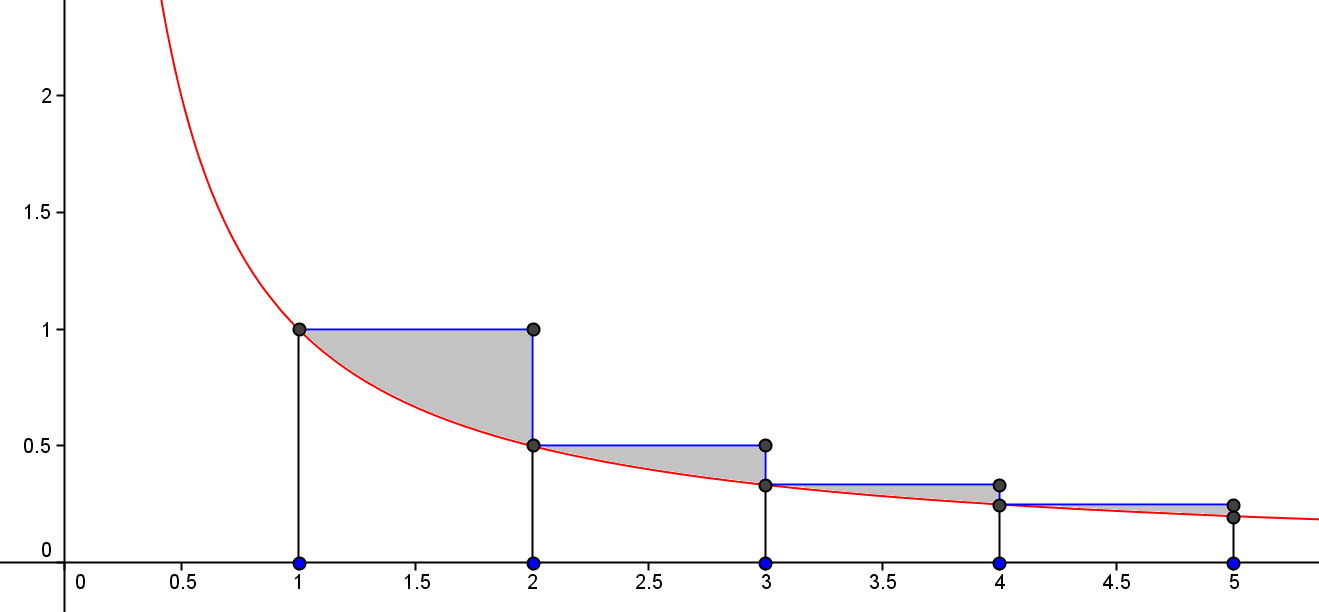
\includegraphics[width=\textwidth]{images/armonica.png}
Fissato un \(N\), intero, vale sempre 
\[ \int_1^N \frac{1}{n} dx  < \sum_{n=1}^{N-1} \frac{1}{n}\]
Poiché
\[ \int_1^N \frac{1}{n} dx = logN \to +\infty \quad N\to +\infty \]
anche
\[  \sum_{n=1}^{N-1} \frac{1}{n} \to +\infty \quad N \to +\infty \]

\subsection{Condizione necessaria per la convergenza}
Condizione necessaria affinché una serie \(\displaystyle \sum_{n=0}^+\infty\)
converga è che \( a_n \to 0\). Tuttavia non è sufficiente. Esempio: serie armonica \(\displaystyle \sum_{n=1}^{+\infty} \frac{1}{n}\)

\subsection{Serie a termini non negativi}
La successione delle somme parziali è crescente
\[
s_{n+1} = s_n + a_{n+1} \geq s_n
\]
Per il teorema sull'esistenza del limite per successioni monotone, esiste 
\[
\lim_{n \to +\infty} s_n
\]
tale limite sarà finito oppure $+\infty$. Perciò avremo che
\[
\sum_{n=0}^{+\infty} a_n, \quad a_n \geq 0
\]
sarà sempre regolare, ossia sarà o convergente o divergente a $+\infty$

\subsection{Criteri di congruenza}
\subsubsection{Criterio del confronto (*)}
Siano \(\{ a_n \}, \{ b_n \}\) due successioni tali che \(0 \leq a_n \leq b_n\). Se \(\displaystyle \sum_{n=0}^{+\infty} b_n\) converge, allora anche \(\displaystyle \sum_{n=0}^{+\infty} a_n\) converge. Se \(\displaystyle \sum_{n=0}^{+\infty} a_n\) diverge, allora diverge anche \(\displaystyle \sum_{n=0}^{+\infty} b_n\)
\textbf{Dimostrazione}\newline
Siano \(\displaystyle A_n = \sum_{k=0}^{n} a_k\) e \(\displaystyle B_n = \sum_{k=0}^{n} b_k\) con \( A_n \leq B_n \wedge B_n \to B\)
poiché \(A_n \uparrow\)
\[
\exists \lim_{n \to +\infty} A_n = A \leq B \quad \text{con} \quad A \in \mathbb{R}
\]
per il teorema del confronto per successioni \(A=B\)

\subsubsection{Corollario (confronto asintotico) (*)}
Siano \(\{ a_n \}, \{ b_n \}\) successioni positive, tali che \(a_n \sim b_n\)  per \(n \to +\infty\) allora
\[
\sum_{n=0}^{+\infty} a_n \quad \text{converge} \quad \Leftrightarrow \sum_{n=0}^{+\infty} b_n \quad \text{converge}
\]
Hanno cioè lo stesso carattere.
\newpage
\textbf{Dimostrazione}\newline
Poiché \(a_n \sim b_n\)  per \(n \to +\infty\) si ha che
\[
\forall \varepsilon > 0 \quad 1 - \varepsilon < \frac{a_n}{b_n} < 1 + \varepsilon
\]
posto \(\varepsilon = \frac{1}{2}\)
\[
\frac{1}{2} < \frac{a_n}{b_n} < \frac{3}{2}
\]
\[
\frac{1}{2}b_n < a_n< \frac{3}{2}b_n
\]
per il criterio del confronto, la prima disuguaglianza implica che se \(\displaystyle \sum_{n=0}^{+\infty} a_n\) converge, anche \(\displaystyle \sum_{n=0}^{+\infty} b_n\), mentre la seconda che se \(\displaystyle \sum_{n=0}^{+\infty} a_n\) diverge anche \(\displaystyle \sum_{n=0}^{+\infty} b_n\) diverge

\subsubsection{Criterio del rapporto}
Sia \(\{ a_n \}, a_n \geq 0, a_n \neq 0\) definitivamente. Se esiste
\[
\lim_{n \to +\infty} \frac{a_{n+1}}{a_n} = \begin{cases}
l<1 \quad \sum_{n=0}^{+\infty} a_n \quad \text{converge}\\
l=1 \quad \text{nulla si può dire}\\
l>1 \quad \sum_{n=0}^{+\infty} a_n \quad \text{diverge}\\
\end{cases}
\]

\subsubsection{Criterio della radice (*)}
Sia \(\{ a_n \}, a_n \geq 0\). Se esiste
\[
\lim_{n \to +\infty} \sqrt[n]{a_n} = \begin{cases}
l<1 \quad \sum_{n=0}^{+\infty} a_n \quad \text{converge}\\
l=1 \quad \text{nulla si può dire}\\
l>1 \quad \sum_{n=0}^{+\infty} a_n \quad \text{diverge}
\end{cases}
\]
\textbf{Dimostrazione}
\begin{itemize}
  \item $l<1$
  \[
  \lim_{n \to +\infty} \sqrt[n]{a_n} = l < 1
  \]
  allora 
  \[
  \forall \varepsilon > 0 \quad \sqrt[n]{a_n} \leq l + \frac{\varepsilon}{2}
  \]
  ma $l<1$, quindi per un opportuno $\varepsilon > 0$ anche $l< 1 - \varepsilon$. Per cui
  \[
  \sqrt[n]{a_n} \leq l + \frac{\varepsilon}{2} < (1-\varepsilon)+\frac{\varepsilon}{2} = 1 - \frac{\varepsilon}{2}
  \]
  \[
  a_n < \left(1 - \frac{\varepsilon}{2} \right)^n
  \] 
  per il criterio del confronto con la serie geometrica convergente 
  \[
  \sum_{n=1}^{+\infty} \left(1 - \frac{\varepsilon}{2} \right)^n
  \]
  la serie di partenza converge.
  \item $l>1$
  \[
  \lim_{n \to +\infty} \sqrt[n]{a_n} = l > 1
  \]
  analogamente
  \[
  a_n > \left(1 + \frac{\varepsilon}{2} \right)^n \quad \varepsilon>0
  \]
  per il criterio del confronto con la serie geometrica divergente
  \[
  \sum_{n=1}^{+\infty} \left(1 + \frac{\varepsilon}{2} \right)^n
  \]
  la serie di partenza diverge
\end{itemize}

\subsection{Serie a termini di segno qualunque (*)}
Una serie \(\displaystyle \sum_{n=0}^{+\infty} a_n\) si dirà assolutamente convergente se converge \(\displaystyle \sum_{n=0}^{+\infty} |a_n|\). \newline
Se la serie \(\displaystyle \sum_{n=0}^{+\infty} a_n\) converge assolutamente, allora converge. \newline
\textbf{Dimostrazione}
\[
a_n^+ = Max\{ a_n, 0 \}, \quad a_n^- = Max\{ -a_n, 0 \}
\]
\[
a_n = a_n^+ - a_n^-
\]
\[
0\leq a_n^+, \quad a_n^- \leq |a_n|
\]
per il teorema del confronto \(\displaystyle \sum_{n=0}^{+\infty} a_n^+ , \sum_{n=0}^{+\infty} a_n^-\) convergono, quindi
\[
\sum_{n=0}^{+\infty} a_n = \sum_{n=0}^{+\infty} (a_n^+ -a_n^-) \quad \text{converge}
\]

\subsection{Serie a termini di segno alterno}
\[
\sum_{n=0}^{+\infty}(-1)^n a_n \quad \text{con} \quad a_n \geq 0 \quad \forall n
\]
\subsection{Criterio di Leibniz}
Sia data \(\displaystyle \sum_{n=0}^{+\infty}(-1)^n a_n \) tale che \(a_n \geq 0\). Se
\begin{enumerate}
  \item $a_n \downarrow$
  \item $\displaystyle \lim_{n \to +\infty} a_n = 0$
\end{enumerate}
Allora \(\displaystyle \sum_{n=0}^{+\infty}(-1)^n a_n\) converge

\end{document}
